% ============================================================
%  Retrieval Methodology  \input{methodology} in main paper
%
%  Required packages in preamble:
%    \usepackage{algorithm}
%    \usepackage{algpseudocode}   % from the algorithmicx bundle
%    \usepackage{amsmath}
%    \usepackage{booktabs}
%    \usepackage{multirow}
%    \usepackage{makecell}        % for \makecell in confusion matrix headers
%    \usepackage{pifont}          % for \ding{51} / \ding{55}
% ============================================================

\newcommand{\cmark}{\ding{51}}%  checkmark
\newcommand{\xmark}{\ding{55}}%  crossmark

\section{Methodology}
\label{sec:methodology}

We describe three mechanisms, all instantiating a common pattern of offline strategy discovery + online query-conditioned routing:

\paragraph{TC-Chunking} (Section~\ref{sec:indexing-methodology}):
per-cluster selection of a document segmentation strategy ($\mathcal{S}_{\text{chunk}}$) on
\textit{Les Débats}.
\paragraph{TC-Metadata selection} (Section~\ref{sec:metadata-methodology}):
per-cluster selection of a retrieval-time metadata strategy  : filter, rerank, hybrid ($\mathcal{S}_{\text{meta}}$) on the same collection.
\paragraph{Structured retrieval} (Section~\ref{sec:two-phase}):
a supervised query-routing classifier (QRe) followed by a
uniform multi-source allocator (UMS) that controls how the
retrieval budget is distributed across collections.

\subsection{Experimental setup.}
\label{sec:experimental-setup}
All dense embeddings (documents and queries) are produced by Cohere
\texttt{embed-v4.0} via the Cohere API and stored in three independent
ChromaDB collections (one per corpus) under cosine distance. The
clustering pipeline of the TC-* methods reduces training-question
embeddings to 10 dimensions with UMAP~\cite{umap} and clusters them with
HDBSCAN~\cite{hdbscan} (\texttt{min\_cluster\_size}{=}5). The
query-routing classifier is an \texttt{sklearn} logistic regression with
default hyperparameters. The metadata schema, chunking regexes, and
cluster labels were drafted offline by Anthropic Claude Opus on debate samples and validated by a domain historian before
being frozen into the pipeline; no LLM call occurs at indexing or query
time. External baselines (HippoRAGv2~\cite{hipporagv2},
LinearRAG~\cite{linearrag_2025}) are adapted from the authors' reference
implementations with their default hyperparameters, the same Cohere
embeddings, and the same Chroma collections. Full reproducibility
details are in Appendix~\ref{sec:appendix-experimental-setup}.

% The first two share the same UMAP transform~$T$, the same set of
% centroids~$\{\mu_c\}$, and the same nearest-centroid inference rule
% (Algorithm~\ref{alg:tc-inference}); only the strategy set
% $\mathcal{S}$ and the strategy map $s^{*}$ differ.
% Section~\ref{sec:joint-methodology} studies the joint
% $\mathcal{S}_{\text{chunk}}\times\mathcal{S}_{\text{meta}}$ space to
% test whether the two index-side axes interact.


% All three contributions instantiate a common pattern : query-conditioned indexing and retrieval, offline, we discover a small
% set of semantic question clusters and learn, per cluster, the strategy that
% maximises retrieval performance; online, each incoming query is routed via
% nearest-centroid assignment to the corresponding pre-built configuration.
% The heavy computation  index construction, cluster discovery, strategy
% selection  is amortised offline; the online cost reduces to a single
% embedding, a UMAP~\cite{umap} projection, and a nearest-neighbour lookup over at most a
% few dozen centroids.

% We apply this pattern to three decision points along the RAG pipeline.
% Section~\ref{sec:indexing-methodology} addresses \emph{chunking granularity}:
% which segmentation of the source documents best serves each cluster of
% questions. Section~\ref{sec:metadata-methodology} addresses
% \emph{retrieval-time metadata}: which structural filters and rerankers best
% serve each cluster. Section~\ref{sec:joint-methodology} studies the
% \emph{joint} optimisation of these two index-side axes, asking whether their
% contributions are separable or interact. Section~\ref{sec:two-phase} moves
% to the retrieval side and addresses \emph{source selection} at a finer
% granularity: a per-query classifier predicts which collections contain the
% evidence needed to answer the query, complementing the cluster-level
% routing of the index-side mechanisms.
 
% Throughout Sections~\ref{sec:indexing-methodology}–\ref{sec:joint-methodology},
% per-cluster strategy variation is restricted to \textit{Les Débats}, the most
% structurally complex collection; newspaper collections retain article-level
% segmentation and default retrieval, and are only revisited on the retrieval
% side in Section~\ref{sec:two-phase}.

%------------------------------------------------------------



%------------------------------------------------------------
\subsection{Task-Conditioned clustering}
\label{sec:indexing-methodology}

Standard RAG pipelines apply a single document segmentation strategy globally, an \emph{one-size-fits-all} assumption that ignores the structural diversity of
historical questions : a comparative budget question and a biographical bridge-entity question might require evidence at different granularities.
We investigate a task-conditioned indexing framework that selects the
segmentation best suited to each question category, without any per-query
re-indexing overhead.
Re-chunking is restricted to \textit{Les Débats}, the most structurally complex
collection; newspaper collections retain article-level segmentation throughout.

%------------------------------------------------------------
\subsubsection{Chunking Strategy Families}
\label{sec:chunking-families}

We define fourteen strategies in four families (Table~\ref{tab:chunking-families}).
Group~A provides flat baselines, including the production strategy
\texttt{10000\_hierarchical}, which uses ALL-CAPS section headers as structural
anchors before applying a recursive character splitter.
Groups~B and~C exploit \textit{Les Débats}-specific markup: speaker-turn
delimiters (\texttt{M.~[Name].}) and procedural markers (vote resolutions,
amendment lifecycle events) respectively.
Group~D adds agenda-level topic boundaries; \texttt{noVotes} variants strip
deputy roll-call name-lists, which otherwise introduce retrieval noise for
semantic queries.

\begin{table}[htbp]
\centering
\small
\resizebox{\columnwidth}{!}{%
\begin{tabular}{l l p{3.1cm}}
\toprule
\textbf{Group} & \textbf{Strategy} & \textbf{Boundary signal} \\
\midrule
\multirow{2}{*}{A — Baseline}
  & \texttt{10000\_hier.}\textsuperscript{†} & Section headers + recursive splitter \\
  & \texttt{fixed\_\{500,1k,2k,10k\}} & Character windows only \\
\midrule
\multirow{3}{*}{B — Speaker}
  & \texttt{S2\_atomic} & One segment per speaker turn \\
  & \texttt{S3\_window3} & Sliding 3-turn window \\
  & \texttt{S4\_president} & Presidential interventions \\
\midrule
\multirow{2}{*}{C — Procedural}
  & \texttt{S8\_vote} & Vote resolution markers \\
  & \texttt{S10\_amendment} & Amendment lifecycle \\
\midrule
\multirow{4}{*}{D — Topic}
  & \texttt{S9\_topic} & Agenda-item transitions \\
  & \texttt{S9\_topic\_noVotes} & Agenda + vote-list removal \\
  & \texttt{S11\_hybrid} & Topic outer / speaker-turn inner \\
  & \texttt{S11\_hybrid\_noVotes} & Hybrid + vote-list removal \\
\bottomrule
\multicolumn{3}{l}{\footnotesize\textsuperscript{†}~Production baseline.}
\end{tabular}
}
\caption{Fourteen chunking strategies evaluated on \textit{Les Débats}
(1887 corpus), grouped by boundary signal type.
Only this collection is re-chunked; newspaper collections retain
article-level segmentation.}
\label{tab:chunking-families}
\end{table}

Full implementation details, regex patterns, splitter configurations, and chunk
statistics for all fourteen strategies are given in
Appendix~\ref{sec:appendix-chunking} (Table~\ref{tab:chunking-strategies}).

%------------------------------------------------------------
\subsubsection{Cluster-Based Strategy Assignment at Inference}
\label{sec:indexing-inference}

In practice, we need a mechanism to assign an unseen query
to a cluster at inference time and route it to the corresponding pre-built index. The framework is zero-shot in the sense that question-type labels can be predicted
directly from the query text without labelling
individual queries for the strategy selector.


\paragraph{Training.}
Training questions are embedded, reduced and clustered to obtain semantic question groups.
For each cluster $c$ (including the HDBSCAN noise group, label $-1$), all
fourteen segmentation strategies are scored by Coverage@3 using the Naive
Retriever ($k_0{=}3$, matching the evaluation budget); the best-scoring
strategy $s^{*}(c)$ is recorded.


\paragraph{Inference.}
At query time, the test question $q$ is embedded and projected into the training
UMAP space via $T$.
The nearest centroid by Euclidean distance determines the cluster assignment
$\hat{c}_q = \arg\min_{c}\;\|\mathbf{z}_q - \mu_c\|_2$.
The query is then served from the pre-built index for strategy $s^{*}(\hat{c}_q)$
and retrieval proceeds with the Retriever at budget $k$.
The marginal online cost is one UMAP projection and one nearest-neighbour
lookup over $|\{\mu_c\}|$ centroids, negligible compared to embedding.
Algorithm~\ref{alg:tc-inference} summarises both phases.



\begin{algorithm}[htbp]
\caption{Task-Conditioned Indexing: Training \& Inference}
\label{alg:tc-inference}
\small
\begin{algorithmic}[1]
\Statex \textbf{Training phase}
\Require Training questions $\mathcal{Q}_{\text{train}}$, strategy set $\mathcal{S}$,
         budget $k_0{=}3$
\Ensure  UMAP transform $T$, centroids $\{\mu_c\}$, strategy map $s^{*}$
\State $T,\; Z \leftarrow \textsc{UMAPFit}\bigl(\textsc{Embed}(\mathcal{Q}_{\text{train}}),\; d{=}10\bigr)$
    \Comment{fit reducer; $Z$ holds the 10-D projections}
\State $\{\ell_q\} \leftarrow \textsc{HDBSCAN}(Z)$
    \Comment{cluster labels; $\ell_q{=}{-}1$ = noise group}
\For{each cluster $c$ (including noise group $-1$)}
    \State $\mathcal{Q}_c \leftarrow \{q \in \mathcal{Q}_{\text{train}} \mid \ell_q = c\}$
    \State $\mu_c \leftarrow \mathrm{mean}\{Z[q] : q \in \mathcal{Q}_c\}$
        \Comment{centroid in UMAP space}
    \State $s^{*}(c) \leftarrow \displaystyle\arg\max_{s \in \mathcal{S}}\;
            \textsc{Cov@}k_0\!\bigl(\textsc{Retrieve}(\mathcal{Q}_c,\, s,\, k_0)\bigr)$
\EndFor
\Statex
\Statex \textbf{Inference phase}
\Require Test query $q$, transform $T$, centroids $\{\mu_c\}$, map $s^{*}$, budget $k$
\Ensure  Ranked list $L$ of $k$ documents
\State $\mathbf{z}_q \leftarrow T\bigl(\textsc{Embed}(q)\bigr)$
    \Comment{project query into UMAP space}
\State $\hat{c} \leftarrow \arg\min_{c}\; \|\mathbf{z}_q - \mu_c\|_2$
    \Comment{nearest training centroid}
\State \Return $\textsc{Retrieve}(q,\, s^{*}(\hat{c}),\, k)$
\end{algorithmic}
\end{algorithm}

% \begin{algorithm}[htbp]
% \caption{Task-Conditioned Indexing. \textsc{UMAPFit} reduces query
% embeddings to $d{=}10$; HDBSCAN label $-1$ is treated as a regular
% cluster; $k_0{=}3$ matches the evaluation budget.}
% \label{alg:tc-inference}
% \small
% \begin{algorithmic}[1]
% \Statex \textbf{Training}
% \Require $\mathcal{Q}_{\text{train}}$, strategy set $\mathcal{S}$, budget $k_0$
% \Ensure  $T$, $\{\mu_c\}$, $s^{*}$
% \State $T,\; Z \leftarrow \textsc{UMAPFit}\bigl(\textsc{Embed}(\mathcal{Q}_{\text{train}})\bigr)$
% \State $\{\ell_q\} \leftarrow \textsc{HDBSCAN}(Z)$
% \For{each cluster $c$}
%     \State $\mathcal{Q}_c \leftarrow \{q : \ell_q = c\}$;\;\;
%            $\mu_c \leftarrow \mathrm{mean}\{Z[q] : q \in \mathcal{Q}_c\}$
%     \State $s^{*}(c) \leftarrow \displaystyle\arg\max_{s \in \mathcal{S}}\;
%             \textsc{Cov@}k_0\!\bigl(\textsc{NaiveRetrieve}(\mathcal{Q}_c,\, s,\, k_0)\bigr)$
% \EndFor
% \Statex \textbf{Inference} \Comment{query $q$, budget $k$}
% \State $\mathbf{z}_q \leftarrow T\bigl(\textsc{Embed}(q)\bigr)$;\;\;
%        $\hat{c} \leftarrow \arg\min_{c}\; \|\mathbf{z}_q - \mu_c\|_2$
% \State \Return $\textsc{NaiveRetrieve}(q,\, s^{*}(\hat{c}),\, k)$
% \end{algorithmic}
% \end{algorithm}


% \paragraph{Evaluation protocol.}
% We compare each task-conditioned configuration against a fixed global baseline (\texttt{10000\_hierarchical} applied uniformly across all queries) using the
% 50/50 split described above, with $n_{\text{train}}{=}437$ and
% $n_{\text{test}}{=}438$ per seed. HDBSCAN produces roughly 29 semantic clusters
% along with a noise group, and all of them participate in strategy selection on
% equal footing. For significance analysis, we train a nearest-centroid classifier
% on the 50/50 question split across 5 random seeds. The full procedure is
% detailed in Algorithm~\ref{alg:tc-inference}. Extended per-cluster results and
% qualitative analysis appear in Appendices~\ref{sec:appendix-clustering-eval}
% and~\ref{sec:appendix-cluster-findings}.


\paragraph{Evaluation protocol (shared across §\ref{sec:indexing-methodology}--\ref{sec:metadata-methodology}).}
We compare each task-conditioned configuration against a fixed global baseline (\texttt{10000\_hierarchical} applied uniformly across all queries) using a 50/50 split, with $n_{\text{train}}{=}437$ and $n_{\text{test}}{=}438$ per seed, repeated across 5 random seeds for significance.
HDBSCAN produces semantic clusters plus a noise group, all participating in strategy selection on equal footing. Extended per-cluster results and qualitative analysis appear in Appendices~\ref{sec:appendix-clustering-eval} and~\ref{sec:appendix-cluster-findings}.
% \begin{figure}[t]
% \centering
% \includegraphics[width=\linewidth]{images/tc_umap_clusters.pdf}
% \caption{2D UMAP projection of training questions (cosine distance metric),
% coloured by each cluster's optimal chunking strategy.
% The embedding space self-organises into semantically coherent regions:
% clusters dominated by amendment debates (orange) favour \texttt{S10\_amendment};
% comparative editorial questions (green) favour \texttt{S9\_topic\_noVotes};
% heterogeneous procedural debates (blue) favour the large-window baseline.
% Cluster ids match those in Table~\ref{tab:cluster-best-chunking}.}
% \label{fig:tc-umap}
% \end{figure}

%------------------------------------------------------------
\subsection{Task-Conditioned Metadata Indexing}
\label{sec:metadata-methodology}

Chunking sets the \emph{granularity} of indexed units. A second, orthogonal
axis controls \emph{which units} are eligible or how they are re-ranked,
via structural metadata (document type, speaker count, document length).

The UMAP transform $T$, centroids $\{\mu_c\}$, split, and inference rule of Algorithm~\ref{alg:tc-inference} are reused unchanged, only the strategy set $\mathcal{S}$ and the map $s^{*}$ change. The metadata pipeline is still restricted to \textit{Les Débats} (newspaper retrieval is left unchanged) and operates on top of the global \texttt{10000\_hierarchical} index.

We define fourteen strategies in three families (Appendix Table~\ref{tab:metadata-strategies}): \textbf{filter} strategies
pre-restrict the index with a Boolean predicate over metadata,
\textbf{rerank} strategies re-score the retrieved candidates with a
multiplicative boost, and \textbf{hybrid} strategies compose both. The
\texttt{baseline} is unconditional retrieval. Full implementation details (predicates, $\alpha$ values, type-set definitions) are given in Appendix~\ref{sec:appendix-metadata}


\subsection{Structured Retriever}
\label{sec:two-phase}

% \begin{figure*}[t]
%   \centering
%   %\hspace{-2.3cm}
%   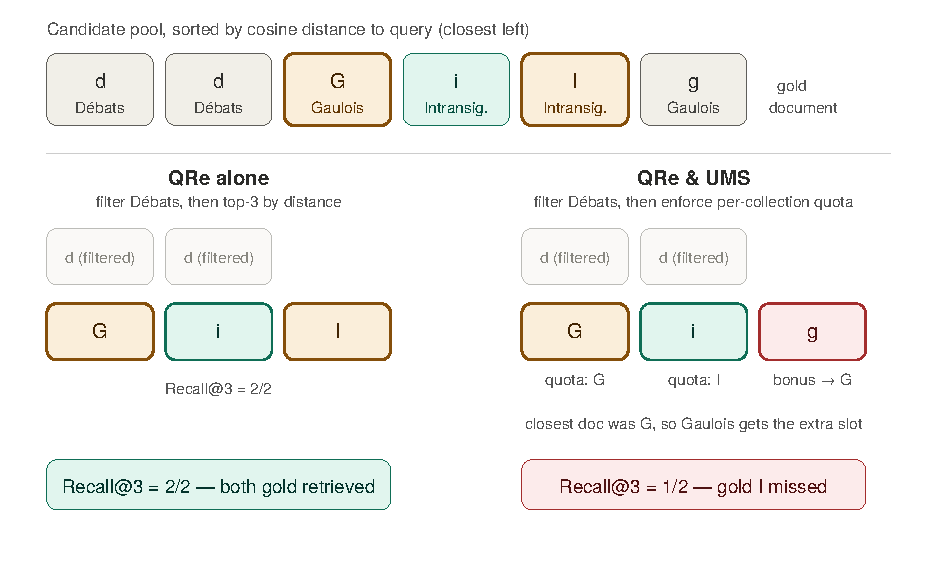
\includegraphics[width=1\textwidth]{images/qre_ums_example_compact.pdf}
%   \caption{TO DO}
%   \label{fig:teaser}
% \end{figure*}

We evaluate four retrieval strategies for multi-source and multi-hop question answering
over three heterogeneous historical corpora: \textit{Le Gaulois} (newspaper),
\textit{L'Intransigeant} (newspaper), and \textit{Les Débats} (parliamentary
transcripts from the French Chambre des Députés), each indexed as an independent
dense vector store (Appendix~\ref{sec:appendix-experimental-setup}).

For each question $q$, we first embed it into a dense vector
$\mathbf{v}_q = \textsc{Embed}(q)$.
This embedding plays two distinct roles in what follows:
(i) it is the input to a supervised query-routing classifier $f_\theta$
that predicts a source-pair label
$\hat{y}_q = f_\theta(\mathbf{v}_q)$, which a routing map $\phi$ then
turns into a set of \emph{active} collections $\mathcal{A}_q = \phi(\hat{y}_q)$
(Section~\ref{sec:classifier}); and (ii) it is the query vector used at
retrieval time to rank documents by cosine distance within each collection.
The four strategies of Section~\ref{sec:retrieval-strategies} differ only in
which collections are queried (all of $\mathcal{C}$ vs.\ only $\mathcal{A}_q$)
and how the budget $k$ is split across them; each strategy issues its own
top-$k$ requests to the relevant collection indices and returns a ranked list
of exactly $k$ documents. Every retrieved document $d$ is annotated with
$\textsc{source}(d)$, the collection it was retrieved from.




%------------------------------------------------------------
\subsubsection{Query Routing via Supervised Classification}
\label{sec:classifier}

We train a classifier $f_\theta$ that predicts, from a question alone, which
collection types contain the evidence needed to answer it.
The model is a logistic regression over the query embedding $\mathbf{v}_q$,
trained on a separate sample of 500 multi-hop questions with
labelled source-pair annotations.
Given the query embedding $\mathbf{v}_q$, it produces a predicted source-pair
label
\begin{equation}
  \label{eq:classifier}
  \hat{y}_q \;=\; f_\theta(\mathbf{v}_q) \;\in\;
  \{\,\texttt{G+I},\; \texttt{I+D},\; \texttt{G+D}\,\},
\end{equation}
corresponding to the three source-pair classes
\textit{Le Gaulois} $+$ \textit{L'Intransigeant} (\texttt{G+I}),
\textit{L'Intransigeant} $+$ \textit{Les Débats} (\texttt{I+D}), and
\textit{Le Gaulois} $+$ \textit{Les Débats} (\texttt{G+D}).
On the held-out test set ($n{=}177$), raw 3-class accuracy is 80.2\%.

\paragraph{The 3-class problem is effectively binary.}
Inspection of the 3-class confusion matrix (Appendix Table~\ref{tab:confusion}) reveals a characteristic error
structure: the two classes that both involve \textit{Les Débats} (\texttt{I+D}
and \texttt{G+D}) are systematically confused with each other, while neither
is ever misclassified as the newspaper-only class \texttt{G+I}, and only one
\texttt{G+I} question is misrouted to a \textit{Les Débats} class.
The internal \texttt{I+D}/\texttt{G+D} ambiguity is irrelevant for retrieval,
since both classes activate the same set of collections (all three corpora).
Collapsing the 3-class output to the binary decision \emph{``does this question
require \textit{Les Débats}?''} yields 99.4\% accuracy on the held-out
test set (176/177 correct: 114/114 on \textit{with Les Débats}, 62/63 on
newspapers-only; see Table~\ref{tab:confusion-binary} in
Appendix~\ref{sec:appendix-classifier}).
Full classifier details, training setup, and error analysis are reported in
Appendix~\ref{sec:appendix-classifier}.

A routing map $\phi$ converts the predicted label $\hat{y}_q$ from
Eq.~\ref{eq:classifier} into a set of active collections
$\mathcal{A}_q$, using shorthands $\mathcal{G}$, $\mathcal{I}$,
$\mathcal{D}$ for \textit{Le Gaulois}, \textit{L'Intransigeant}, and
\textit{Les Débats} respectively:
%
\begin{equation}
  \label{eq:routing}
  \mathcal{A}_q = \phi(\hat{y}_q) =
  \begin{cases}
    \{\mathcal{G},\, \mathcal{I}\}
      & \text{if } \hat{y}_q = \mathcal{G} + \mathcal{I} \\[4pt]
    \{\mathcal{G},\, \mathcal{I},\, \mathcal{D}\}
      & \text{otherwise}
  \end{cases}
\end{equation}
%
The classifier's effective decision is therefore binary: does the query require
the parliamentary corpus \textit{Les Débats}? Purely newspaper comparative
questions are routed to the two newspaper collections only; questions crossing
newspaper coverage and parliamentary proceedings are routed to all three.

% %------------------------------------------------------------
% \subsubsection{Retrieval Strategies}
% \label{sec:retrieval-strategies}

% All four strategies return a ranked list of exactly $k$ documents and differ
% only along two orthogonal axes: (i) \emph{query routing}  whether retrieval
% is restricted to the set of \emph{active} collections $\mathcal{A}_q$
% predicted by the classifier, and (ii) \emph{uniform quota}  whether the
% budget $k$ is split equally across the collections being queried.
% The \textit{Naive Retriever} uses neither, \textit{QRe} adds routing only,
% \textit{UMS-Retriever} adds the quota only, and \textit{QRe \& UMS-Retriever}
% combines both.
% We denote by $\textsc{topk}(c, k)$ the $k$ documents of collection $c$ with
% smallest cosine distance to $\mathbf{v}_q$.

% \paragraph{Naive Retriever.}
% The default RAG baseline: retrieve from every collection in $\mathcal{C}$ and
% keep the $k$ globally closest documents,
% $L = \textsc{topk}\bigl(\bigcup_{c \in \mathcal{C}} \textsc{topk}(c, k),\, k\bigr)$,
% with no routing and no quota.
% Documents are ranked purely by cosine distance, regardless of source.

% \paragraph{Query Rerouting (QRe).}
% Retrieve only from the active collections $\mathcal{A}_q = \phi(\hat{y}_q)$
% predicted by the classifier, then rank by distance:
% $L = \textsc{topk}\bigl(\bigcup_{c \in \mathcal{A}_q} \textsc{topk}(c, k),\, k\bigr)$.
% Collections deemed irrelevant for $q$ are skipped entirely.

% \paragraph{Uniform Multi-Source Retriever (UMS).}
% Multi-hop questions require evidence from \emph{multiple} sources by
% construction; pure distance ranking can saturate the top-$k$ with documents
% from a single high-scoring collection, starving the others of representation.
% UMS enforces an equal per-source quota over the full collection set
% $\mathcal{C}$: each collection $c$ receives
% \begin{equation}
% \label{eq:quota}
% q_c \;=\; \lfloor k / |\mathcal{C}| \rfloor
%        \;+\; \mathbf{1}\!\bigl[\textsc{rank}(c) \leq k \bmod |\mathcal{C}|\bigr],
% \end{equation}
% where $\textsc{rank}(c)$ orders collections by their closest document's
% distance, so the $k \bmod |\mathcal{C}|$ extra slots go to the globally
% most-relevant collections.
% The final list is the union of $\textsc{topk}(c, q_c)$ over each $c$,
% re-sorted globally by distance.

% \paragraph{QRe \& UMS-Retriever.}
% The two mechanisms compose by applying the UMS quota
% (Eq.~\ref{eq:quota}) over $\mathcal{A}_q$ rather than $\mathcal{C}$:
% the classifier first filters out irrelevant collections, then the remaining
% budget is split equally across the active ones.


\subsubsection{Retrieval Strategies}
\label{sec:retrieval-strategies}

All four strategies return a ranked list of exactly $k$ documents and differ
only along two orthogonal axes: \emph{query routing} (restricting retrieval
to the active collections $\mathcal{A}_q = \phi(\hat{y}_q)$ predicted by the
classifier) and \emph{uniform quota} (splitting $k$ equally across the
queried collections). We denote by $\textsc{topk}(c, k)$ the $k$ documents of
collection $c$ with smallest cosine distance to $\mathbf{v}_q$.

\paragraph{Naive Retriever.}
Default RAG baseline with neither mechanism: retrieve from every collection
in $\mathcal{C}$ and keep the $k$ globally closest documents,
$L = \textsc{topk}\bigl(\bigcup_{c \in \mathcal{C}} \textsc{topk}(c, k),\, k\bigr)$.

\paragraph{Query Rerouting (QRe).}
Routing only: restrict retrieval to $\mathcal{A}_q$ and rank by distance,
$L = \textsc{topk}\bigl(\bigcup_{c \in \mathcal{A}_q} \textsc{topk}(c, k),\, k\bigr)$.

\paragraph{Uniform Multi-Source Retriever (UMS).}
Quota only : since multi-hop questions require evidence from multiple sources,
pure distance ranking can saturate the top-$k$ with a single high-scoring
collection. UMS enforces an equal per-source quota over $\mathcal{C}$:
\begin{equation}
\label{eq:quota}
q_c \;=\; \lfloor k / |\mathcal{C}| \rfloor
       \;+\; \mathbf{1}\!\bigl[\textsc{rank}(c) \leq k \bmod |\mathcal{C}|\bigr],
\end{equation}
where $\textsc{rank}(c)$ orders collections by their closest document's
distance, so the $k \bmod |\mathcal{C}|$ extra slots go to the globally
most-relevant collections. The final list is $\bigcup_c \textsc{topk}(c, q_c)$,
re-sorted by distance.

\paragraph{QRe \& UMS-Retriever.}
The two mechanisms compose by applying the UMS quota
(Eq.~\ref{eq:quota}) over $\mathcal{A}_q$ rather than $\mathcal{C}$:
the classifier first filters out irrelevant collections, then the remaining
budget is split equally across the active ones.
% \subsection{Metrics}

% All questions are multi-hop with exactly two gold documents ($|G_q|{=}2$).
% We report two complementary metrics that differ in their reference unit.

% \paragraph{Recall@k.}
% Recall is \emph{ID-based}: the gold evidence for question $q$ under strategy
% $s$ is a pair of \emph{chunk IDs} $(g_1^s, g_2^s)$ pre-identified in $s$'s
% index; a gold chunk is \emph{found} if its exact ID appears in the top-$k$
% retrieved list $L_q^s$.
% \begin{equation}
% \text{Recall@}k = \frac{1}{|\mathcal{Q}|}\sum_{q \in \mathcal{Q}}
% \frac{\bigl|\{i : g_i^s \in L_q^{(1:k)}\}\bigr|}{2}.
% \end{equation}
% Per-question scores therefore take values in $\{0,\,0.5,\,1\}$: both gold
% chunks missed, one found, or both found.

% \paragraph{Coverage@k.}
% Coverage is \emph{text-based} and handles chunking-granularity asymmetry.
% Let $t_g$ be the text of gold document $g$ (looked up from the index by ID),
% and let $R_q^{s,g} \subseteq L_q^{(1:k)}$ be the retrieved chunks from the
% same source as $g$.
% The per-gold-document score is:
% \begin{equation}
% \sigma(g, R) =
% \begin{cases}
% 1 & \exists\,d{\in}R: t_g \subseteq d, \\[4pt]
% \dfrac{\displaystyle\sum_{d \in R}\mathbf{1}[d \subseteq t_g]\cdot|d|}{|t_g|}
%   & \exists\,d{\in}R: d \subseteq t_g, \\[8pt]
% 0 & \text{otherwise.}
% \end{cases}
% \end{equation}
% Case 1 fires when the gold text is a substring of some retrieved chunk
% (full containment, $\sigma{=}1$); Case 2 accumulates character-level coverage
% when retrieved chunks are substrings of the gold text (partial coverage).
% Coverage@$k$ is then the macro-average of this score over gold documents and
% questions:
% \begin{equation}
% \text{Coverage@}k = \frac{1}{|\mathcal{Q}|}\sum_{q}\frac{1}{2}
% \sum_{g \in G_q} \sigma\!\bigl(g,\, R_q^{s,g}\bigr).
% \end{equation}
% When a strategy produces large chunks (e.g.\ \texttt{10000\_hierarchical}),
% the retrieved chunk often contains the entire gold text and $\sigma{=}1$.
% When chunks are fine-grained, $\sigma$ measures the character-level fraction
% of the gold text covered by the retrieved sub-chunks from the same source.
% Coverage@$k$ is therefore more lenient than Recall@$k$ under coarse-grained
% strategies, and more sensitive to partial evidence under fine-grained ones.


% \subsection{Metrics}
% \label{sec:metrics}

% All questions are multi-hop with exactly two gold documents
% ($|G_q|{=}2$). We report two complementary metrics that differ in
% their reference unit. \textbf{Recall@$k$} is \emph{ID-based}: under
% strategy $s$, each question has a gold pair of chunk IDs
% $(g_1^s, g_2^s)$ pre-identified in $s$'s index, and a gold chunk is
% \emph{found} iff its exact ID appears in the top-$k$ list. Per-question
% scores therefore take values in $\{0,\,0.5,\,1\}$ and are macro-averaged
% over $\mathcal{Q}$. \textbf{Coverage@$k$} is \emph{text-based} and is
% designed to compare strategies that differ in chunk granularity: for
% each gold document $g$ and the retrieved chunks $R \subseteq L_q^{(1:k)}$
% from the same source, the per-document score $\sigma(g, R)$ equals
% $1$ if some retrieved chunk \emph{contains} the gold text (full
% containment), the character-level fraction
% $\sum_{d \subseteq t_g}|d|/|t_g|$ if retrieved chunks are sub-strings
% of $t_g$ (partial coverage), and $0$ otherwise; Coverage@$k$ is the
% macro-average of $\sigma$ over gold documents and questions.
% Coverage is thus strictly more lenient than Recall under coarse
% chunking (one large chunk often contains the entire gold text, giving
% $\sigma{=}1$) and strictly more sensitive than Recall under fine
% chunking (where it credits partial evidence that an ID-match would
% miss). Formal definitions, edge cases, and a worked example are in
% Appendix~\ref{sec:appendix-metrics}.


\subsection{Metrics}
\label{sec:metrics}

All questions are multi-hop with two gold documents. We report two
complementary metrics. \textbf{Recall@$k$} is ID-based: a gold chunk
counts as found iff its exact ID appears in the top-$k$ list, giving
per-question scores in $\{0,\, 0.5,\, 1\}$. \textbf{Coverage@$k$} is
text-based and handles chunking-granularity asymmetry: for each gold
document $g$ and the retrieved chunks $R$ from the same source, the
per-document score is $1$ if some $d \in R$ contains $t_g$, the
character-fraction $\sum_{d \subseteq t_g}|d|/|t_g|$ if retrieved
chunks are sub-strings of $t_g$, and $0$ otherwise; Coverage@$k$ is
the macro-average over gold documents and questions. Coverage is
thus more lenient than Recall under coarse chunking and more
sensitive under fine chunking. Formal definitions, edge cases, and
a worked example are in Appendix~\ref{sec:appendix-metrics}.
